\section{Classification}
\label{s:classification}

Intuitively, we expected the regions in which each algorithm performed better to be highly nonlinear.
As a result, we chose to use a support vector machine for classification, as these are known to have good performance for nonlinear classification~\cite{cortes1995support}.
Specifically, we used MATLAB's~\cite{MATLAB2011} implementation of SVM.
We chose to compare two kernels, the Gaussian radial basis function (RBF)~\cite{buhmann2003radial} and the multilayer perceptron (MLP)~\cite{collobert2004links}.

As described in section~\ref{s:data:gen}, we featurized DMM by using the sizes of the input matrices: M, K, and N.
The output of our classifier is the algorithm that performs better for a given tuple (M, K, N).
The classifier only considers the binary training data---we do not take into account how much better an algorithm performs at each point; we leave this weighted classification to future work.

\subsection{Training}
We trained our classifier on each of our three testing machines.
Our results, shown in Figure~\ref{fig:training}, were surprising.
While we expected some machine-to-machine variation, the regions where each algorithm performs better are substantially different across machines.
Indeed, Emerald and Sandy have diametrically opposed training results.
We do not have a theoretical model to explain this variation, which further illustrates the value of our empirical machine learning approach.
This is a key result: techniques that do not consider per-machine variation are certain to use the wrong algorithm in many cases.
We also note that the regions of optimal performance for each algorithm are in fact nonlinear.

\begin{figure*}[t]
    \centering
        \begin{subfigure}[t]{0.33\textwidth}
            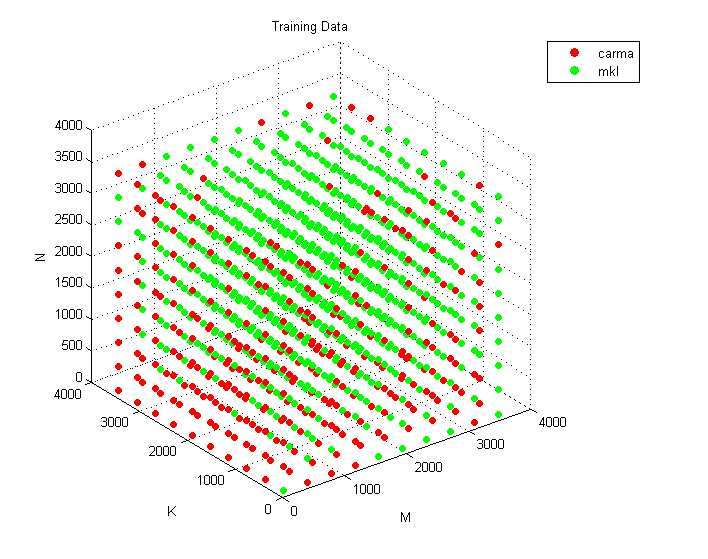
\includegraphics[width=\textwidth]{figures/emerald_train.png}
            \caption{Emerald}
            \label{f:train_emerald}
            \end{subfigure}
        \begin{subfigure}[t]{0.33\textwidth}
            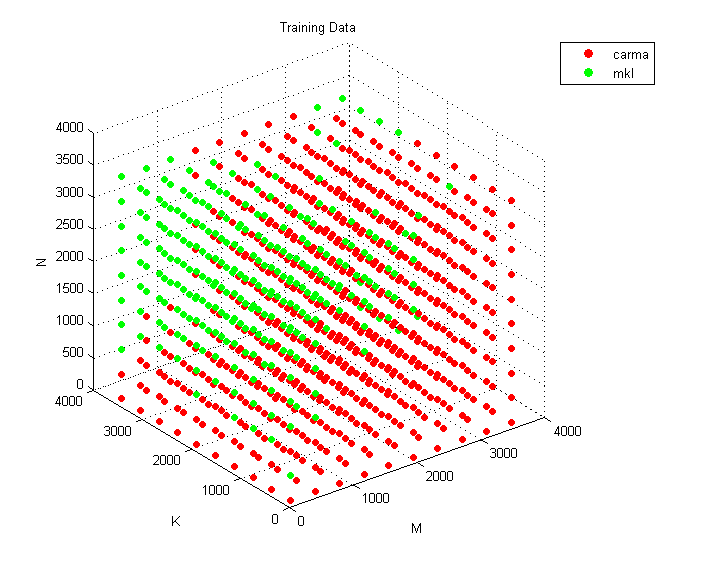
\includegraphics[width=\textwidth]{figures/hopper_train.png}
            \caption{Hopper}
            \label{f:train_hopper}
        \end{subfigure}
        \begin{subfigure}[t]{0.33\textwidth}
            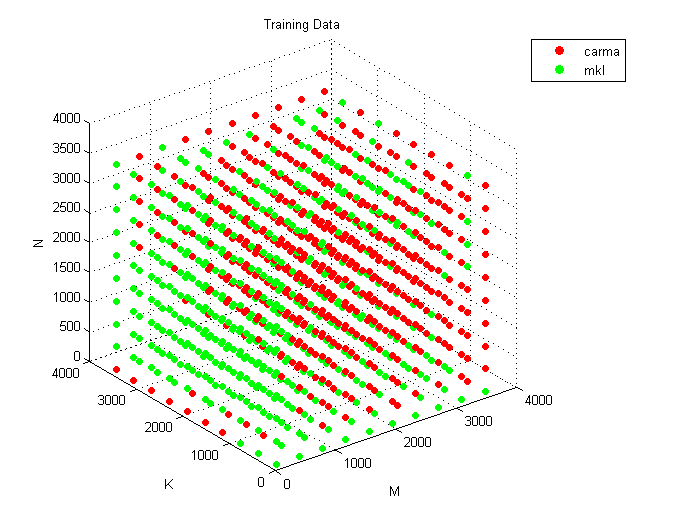
\includegraphics[width=\textwidth]{figures/sandy_train.png}
            \caption{Sandy}
            \label{f:train_sandy}
        \end{subfigure}
        \caption{Training results for each of our three machines. Green dots represent datapoints where MKL outperformed CARMA, red dots indicate the opposite. Note how the results are almost completely reversed for Emerald and Sandy.}
    \label{fig:training}
\end{figure*}

Another surprising result of our training was the fact that CARMA performed well for such large regions.
CARMA's developers had designed it for multiplication of ``long, skinny'' matrices, and it outperformed MKL for those on all three of our machines.
However, its strong performance for other types of matrices was unexpected, and will be analyzed in the future.

\subsection{Classifying}
In order to evaluate our classifier, we needed to generate random datapoints for testing.
We randomly generated values for M, K, and N within our training space, and replicated our data-collecting procedure to time the multiplications and record which algorithm ran faster.
After gathering this test data, we removed the true class labels and ran the values for M, K, and N through our classifier (once per machine for each kernel).
Given the true and predicted label for each testing datapoint, we now had enough information to evaluate our classifier.
See Figure~\ref{fig:classifying} for the results of this procedure.

\begin{figure*}[t]
    \centering
        \begin{subfigure}[t]{0.33\textwidth}
            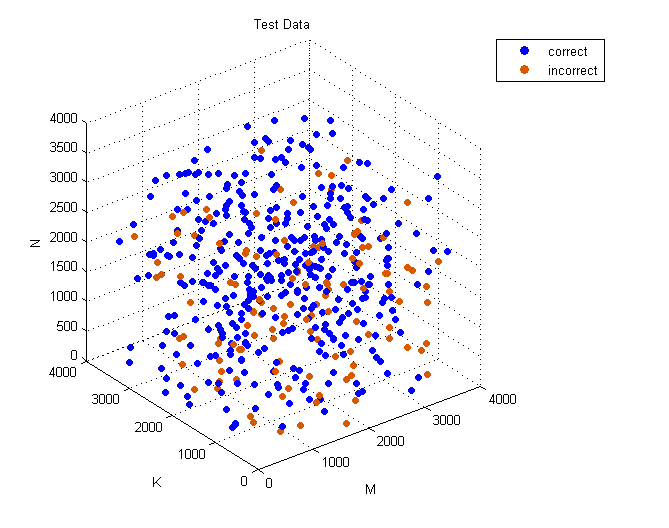
\includegraphics[width=\textwidth]{figures/emerald_test_rbf.png}
            \caption{Emerald - RBF}
            \label{f:classify_rbf_emerald}
        \end{subfigure}
        \begin{subfigure}[t]{0.33\textwidth}
            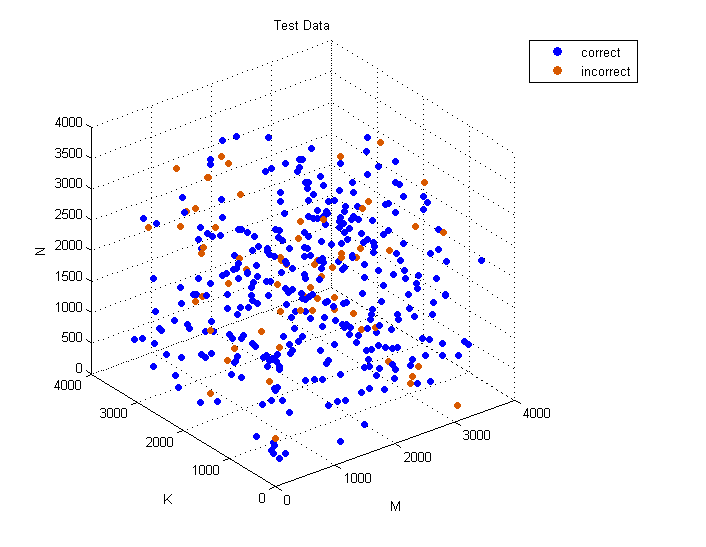
\includegraphics[width=\textwidth]{figures/hopper_test_rbf.png}
            \caption{Hopper - RBF}
            \label{f:classify_rbf_hopper}
        \end{subfigure}
        \begin{subfigure}[t]{0.33\textwidth}
            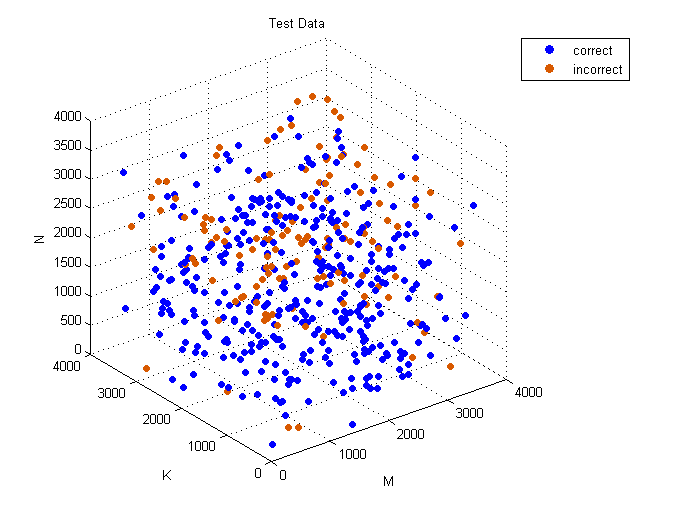
\includegraphics[width=\textwidth]{figures/sandy_test_rbf.png}
            \caption{Sandy - RBF}
            \label{f:classify_rbf_sandy}
        \end{subfigure}
    \centering
        \begin{subfigure}[t]{0.33\textwidth}
            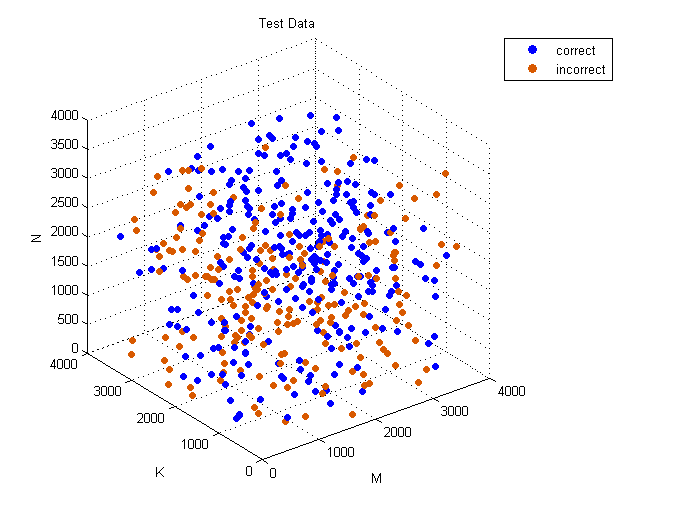
\includegraphics[width=\textwidth]{figures/emerald_test_mlp.png}
            \caption{Emerald - MLP}
            \label{f:classify_mlp_emerald}
        \end{subfigure}
        \begin{subfigure}[t]{0.33\textwidth}
            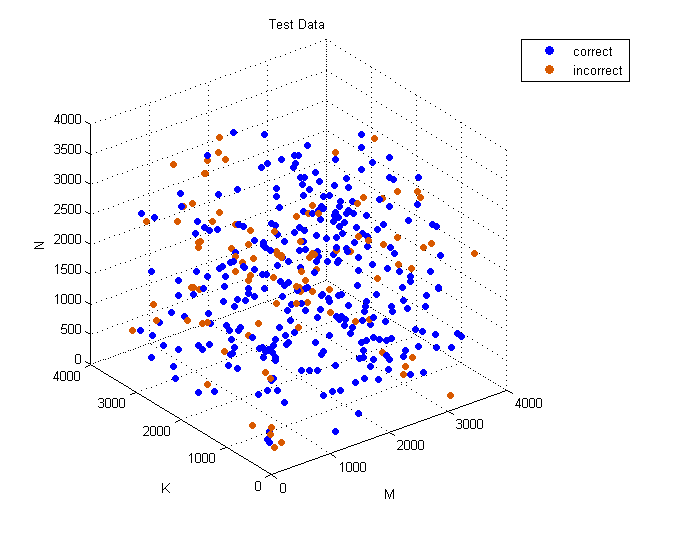
\includegraphics[width=\textwidth]{figures/hopper_test_mlp.png}
            \caption{Hopper - MLP}
            \label{f:classify_mlp_hopper}
        \end{subfigure}
        \begin{subfigure}[t]{0.33\textwidth}
            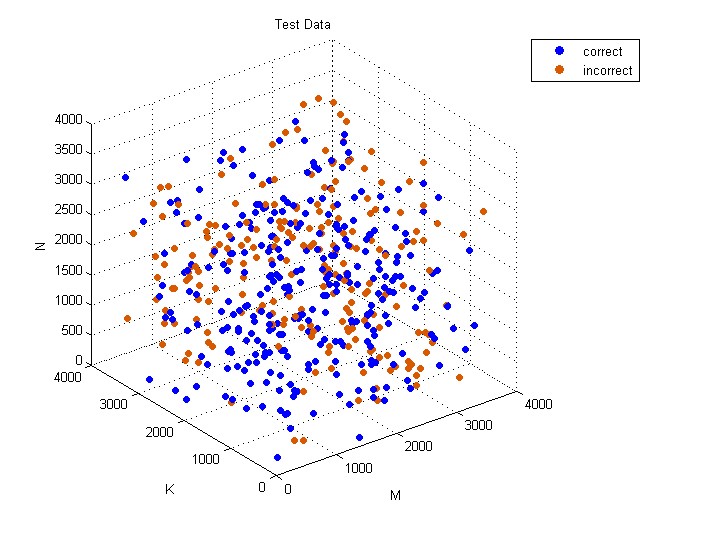
\includegraphics[width=\textwidth]{figures/sandy_test_mlp.png}
            \caption{Sandy - MLP}
            \label{f:classify_mlp_sandy}
        \end{subfigure}

        \caption{Testing results for each of our three machines, for each kernel (RBF and MLP). Blue dots represent datapoints where our classifier correctly predicted which algorithm was faster, and orange dots represent incorrect classifications. Note that the RBF kernel outperforms the MLP kernel on all machines (most significantly on Emerald and Sandy).}
    \label{fig:classifying}
\end{figure*}

It is worth noting that the majority of incorrect classifications occur on or near the decision boundaries our classifier generated.
This is due to the fact that along these decision boundaries, the performance of MKL and CARMA is comparable.
On any given trial, CARMA may slightly outperform MKL, or MKL may marginally beat CARMA.
Therefore, the class that our classifier assigns to datapoints along a decision boundary may not match the given instance of performance data that we gathered, even though the actual performance difference is relatively minor.

To better visualize this phenomenon, we simplified the problem by reducing it to a two-dimensional classification problem.
By only considering datapoints where K = N, we were able to train a 2D classifier to better visualize the decision boundary.
See Figure~\ref{fig:2D}.

\begin{figure*}[t]
    \centering
        \begin{subfigure}[t]{0.49\textwidth}
            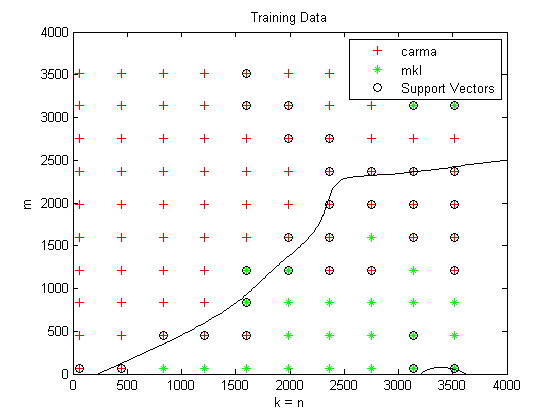
\includegraphics[width=\textwidth]{figures/hopper2D_train_mlp.png}
            \caption{Training: Green dots represent datapoints where MKL outperformed CARMA, red dots indicate the reverse.}
            \label{f:train_hopper_2D}
            \end{subfigure}
        \begin{subfigure}[t]{0.49\textwidth}
            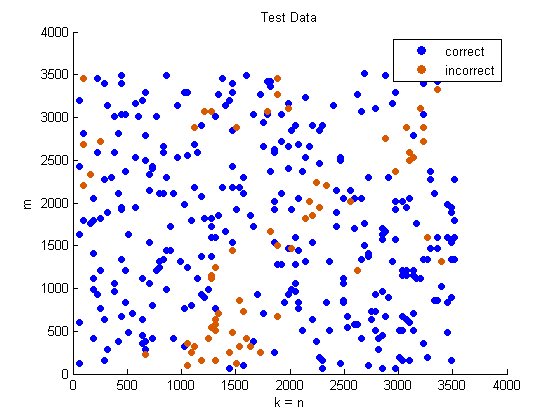
\includegraphics[width=\textwidth]{figures/hopper2D_test_mlp.png}
            \caption{Testing: Blue dots represent datapoints where our classifier correctly predicted which algorithm was faster, and orange dots represent incorrect classifications.}
            \label{f:test_hopper_2D}
        \end{subfigure}
        \caption{Training vs. testing on Hopper using the MLP kernel. Observe that the majority of incorrect classifications (orange dots in subfigure b) occur along the decision boundary, where CARMA and MKL exhibit similar performance behavior.}
    \label{fig:2D}
\end{figure*}

On average, the performance loss resulting from an incorrect classification is only 9.6\%, supporting the observation that the majority of these misclassifications occur along decision boundaries where CARMA's and MKL's performance are comparable.
